\chapter{Pesquisa-ação}
\label{pesquisa_acao}

		A organização a ser tratada como objeto da pesquisa-ação neste trabalho refere-se aos grupos de trabalho das disciplinas de Gestão de Projetos
		e Portfólio (GPP) e Metodologias de Desenvolvimento de Software (MDS), do curso de Engenharia de \textit{Software}
		da Universidade de Brasília.

		\section{Descrição da organização}

			A organização trabalha na produção de software com vários projetos, os quais possuem as seguintes características:

			\begin{itemize}
				\item Uso de dados abertos;
				\item Aplicações WEB e aplicativos \textit{mobile};
				\item Equipe composta de dois times:
					\subitem 1 time de desenvolvimento;
					\subitem 1 equipe de gerência;
				\item Equipes pequenas e inexperientes;
				\item Prazo fixo;
				\item Aplicação da metodologia de desenvolvimento tradicional e da metodologia ágil.
			\end{itemize}

	\section{Diagnóstico}

	Para a realização da pesquisa-ação será considerado um projeto em andamento da organização que possui as seguintes características:


\begin{itemize}
	\item Aplicativo \textit{mobile};
	\item Equipe composta de dois times:
		\subitem 1 time de desenvolvimento com 6 pessoas;
		\subitem 1 equipe de gerência com 6 pessoas;
	\item Membros inexperientes na tecnologia.
	\item Uso de metodologia ágil;
	\item Quantidade de \textit{Sprints}: 7;
	\item Tamanho da \textit{Sprint}: 1 semana;
	\item Dedicação parcial do time, visto que trata-se de uma disciplina.
\end{itemize}



O diagnóstico realizado para ver a situação atual do projeto, selecionado para o estudo, consistiu na análise
	dos gráficos de \textit{Burndown} das quatro primeiras \textit{Sprints} e na aplicação de um questionário para o
	time de desenvolvimento.

	\subsection{Análise dos gráficos de \textit{Burndown}}

	Para as quatro primeiras \textit{Sprints} é possível ver nas Figuras \ref{fig:burndown0}, \ref{fig:burndown1}, \ref{fig:burndown2}
	\ref{fig:burndown3} que os pontos realizados não correspondem a pontuação total planejada para a \textit{Sprint}.
	Assim é possível ver que que nem todas as histórias alocadas foram entregues, o que significa que houve atrasos nas entregas.

	O acompanhamento do \textit{Burndown} por \textit{Sprint} auxiliou na visualização da distribuição do trabalho dentro da \textit{Sprint}.
	Assim foi possível ver, por exemplo, que nas \textit{Sprints} 0 e 1 o time demorou para começar a trabalhar, o que pode ter sido uma causa do atraso. Dessa forma, impactando nas \textit{Sprints} seguintes.

	\begin{figure}[!h]
	\begin{minipage}[b]{0.5\linewidth}
	\centering
	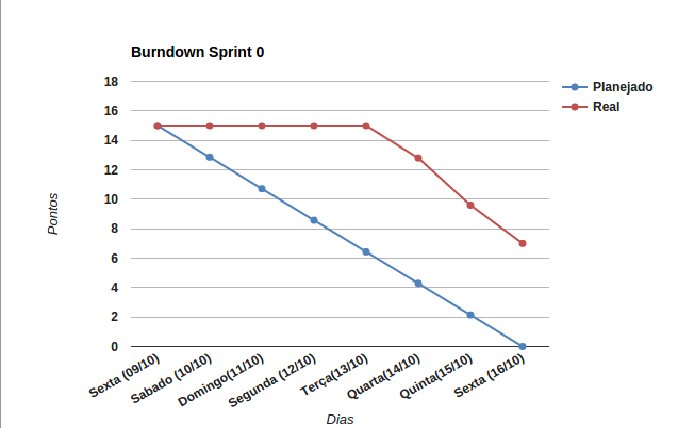
\includegraphics[scale=0.5]{figuras/burndown_sprint0.png}
	\caption{Burndown da \textit{Sprint} 0.}
	\label{fig:burndown0}
	\end{minipage}
	\hspace{0.5cm}
	\begin{minipage}[b]{0.5\linewidth}
	\centering
	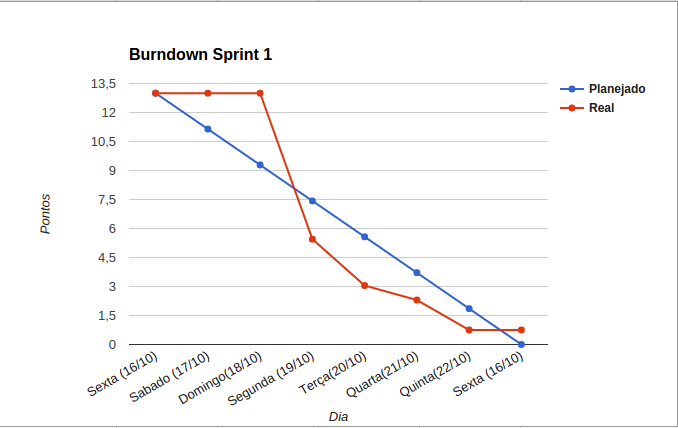
\includegraphics[scale=0.5]{figuras/burndown_sprint1.png}
	\caption{Burndown da \textit{Sprint} 1.}
	\label{fig:burndown1}
	\end{minipage}
	\end{figure}

	\begin{figure}[!h]
	\begin{minipage}[b]{0.5\linewidth}
	\centering
	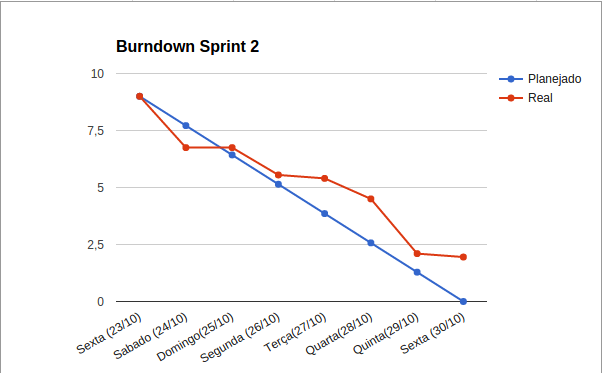
\includegraphics[scale=0.5]{figuras/burndown_sprint2.png}
	\caption{Burndown da \textit{Sprint} 2.}
	\label{fig:burndown2}
	\end{minipage}
	\hspace{0.5cm}
	\begin{minipage}[b]{0.5\linewidth}
	\centering
	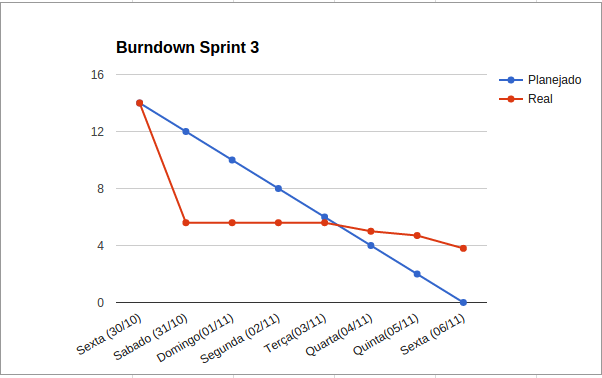
\includegraphics[scale=0.5]{figuras/burndown_sprint3.png}
	\caption{Burndown da \textit{Sprint} 3.}
	\label{fig:burndown3}
	\end{minipage}
	\end{figure}

	\vfill
	\pagebreak

	\subsection{Questionário}

	A fim de coletar dados sobre a percepção dos membros sobre possíveis aspectos que afetaram a entrega nos prazos foi aplicado
	um questionário ao time de desenvolvimento que se encontra no apêndice \ref{apendice:questionario}.

	No apêndice pode ser visto que o questionário é composto de afirmações que são avaliadas pelo respondente em uma escala de 1 a 5. Na qual 1 significa discordância total da afirmação e 5 concordância total.

	As respostas coletadas foram contabilizadas de acordo com cada categoria da escala para cada afirmação. Cada afirmação tratava de um fator que poderia estar ocasionando os atrasos. Essas afirmações são:

	\begin{table}[h!]
	\centering
	\caption{Afirmações do questionário e fatores associados}
	\label{my-label}
	\begin{tabular}{|l|l|}
	\hline
	\multicolumn{1}{|c|}{\textbf{Afirmação}}                                                     & \multicolumn{1}{c|}{\textbf{Fator}}                                                       \\ \hline
	\begin{tabular}[c]{@{}l@{}}1. Os atrasos ocorridos decorreram dos\\  erros nas estimativas em StoryPoints.\end{tabular}                 & Erro nas estimativas                                                                      \\ \hline
	\begin{tabular}[c]{@{}l@{}}2. A dificuldade na linguagem ocasionou\\  os atrasos nas entregas da \textit{Sprint}.\end{tabular}        & Dificuldade na linguagem                                                                  \\ \hline
	\begin{tabular}[c]{@{}l@{}}3. O tamanho da \textit{Sprint}\\  afetou nas entregas no prazo.\end{tabular}                              & Tamanho da \textit{Sprint}                                                              \\ \hline
	\begin{tabular}[c]{@{}l@{}}4. Os atrasos decorreram da mudança\\  de metodologia, devido ao período de adaptação.\end{tabular}          & \begin{tabular}[c]{@{}l@{}}Dificuldade na adaptação \\ para metodologia ágil\end{tabular} \\ \hline
	\begin{tabular}[c]{@{}l@{}}5. A demora na iniciação do desenvolvimento na\\  \textit{Sprint} ocasionou os atrasos.\end{tabular}       & Procrastinação                                                                            \\ \hline
	\begin{tabular}[c]{@{}l@{}}6. A dificuldade na comunicação afetou\\  a entrega no prazo.\end{tabular}                                   & Dificuldade na comunicação                                                                \\ \hline
	\begin{tabular}[c]{@{}l@{}}7. A dedicação parcial do time afetou\\  a entrega no prazo.\end{tabular}                                    & Dedicação parcial do time                                                                 \\ \hline
	\begin{tabular}[c]{@{}l@{}}8. A dificuldade no entendimento das histórias\\  acarretou nos atrasos nas \textit{sprints}.\end{tabular} & \begin{tabular}[c]{@{}l@{}}Dificuldade no entendimento\\  das histórias\end{tabular}      \\ \hline
	\end{tabular}
	\end{table}


	O questionário também continha uma pergunta aberta com resposta opcional. Assim, para essa questão só houve uma resposta, que foi a seguinte:

	\textit{"Acho que o que mais impactou foi a falta de comprometimento com o projeto. Acho que de resto não é tao relevante assim"}

	A sumarização dos resultados das questões afirmativas pode ser vista na Tabela \ref{tab:analise_respostas}.	Para uma melhor visualização das respostas também foram gerados gráficos, que também podem ser vistos em apêndice (Apêndice \ref{apendice:graficos}).

	\begin{table}[!h]
	\flushleft
	\caption{Percentual de respostas por categoria em cada pergunta}
	\label{tab:analise_respostas}
	\begin{tabular}{|c|l|l|l|l|l|l|l|l|}
	\hline
	\textbf{\begin{tabular}[c]{@{}c@{}}Afirmação/\\ Categorias\end{tabular}} & \textbf{1} & \textbf{2} & \textbf{3} & \textbf{4} & \textbf{5} & \textbf{6} & \textbf{7} & \textbf{8} \\ \hline
	\begin{tabular}[c]{@{}c@{}}Discordo\\  totalmente\end{tabular}   & 0\%        & 0\%        & 16,67\%    & 33,33\%    & 0\%        & 0\%        & 16,67\%    & 100\%      \\ \hline
	\begin{tabular}[c]{@{}c@{}}Discordo\\  parcialmente\end{tabular} & 0\%        & 0\%        & 33,33\%    & 33,33\%    & 0\%        & 16,67\%    & 50\%       & 0\%        \\ \hline
	Neutro                                                           & 33,33\%    & 0\%        & 33,33\%    & 33,33\%    & 16,67\%    & 33,3\%     & 16,67\%    & 0\%        \\ \hline
	\begin{tabular}[c]{@{}c@{}}Concordo\\  parcialmente\end{tabular} & 50\%       & 50\%       & 16,67\%    & 0\%        & 66,67\%    & 50\%       & 0\%        & 0\%        \\ \hline
	\begin{tabular}[c]{@{}c@{}}Concordo\\  totalmente\end{tabular}   & 16,67\%    & 50\%       & 0\%        & 0\%        & 16,67\%    & 0\%        & 16,67\%    & 0\%        \\ \hline
	\end{tabular}
	\end{table}



		\subsubsection{Análise das respostas}

			Analisando os dados apresentados na tabela \ref{tab:analise_respostas} e através do acompanhamento das \textit{sprints}, é possível analisar os fatores que a equipe acredita que tenham ocasionado os atrasos.

			Dessa forma, é possível ver que a equipe considera que errou nas estimativas em \textit{StoryPoints} e isso afetou nas entregas das histórias, visto que a maioria respostas convergiu para a concordância com a afirmação. Esse fator é um fator provável dentro da organização considerada nesse trabalho, visto que as equipes são inexperientes.

			Outro fator que convergiu para a concordância foi a dificuldade na linguagem. O time analisa como um grande fator que impediu o desenvolvimento das histórias no prazo.

			O tamanho da \textit{sprint} foi um fator que não houve uma convergência nítida, todavia a maioria discordou ou se colocou como neutro em relação a esse fator. Assim, não é um fator que tem um peso sobre os atrasos ocorridos.

			A adaptação para a nova metodologia não foi um fator responsável pelos atrasos visto que as respostas convergiram para a discordância da afirmação.

			A demora na iniciação do desenvolvimento, ou seja, a procrastinação da equipe foi considerado um fator responsável pelos atrasos, visto que as respostas convergiram para a concordância.

			Em relação à dificuldade na comunicação a equipe se posicionou, em sua maioria, neutra ou em uma concordância parcial. A partir disso é possível
			ver que a dificuldade de comunicação afeta os atrasos mas com um peso bem menor que outros fatores.

			Para o fator dedicação parcial é possível que a equipe, em sua maioria, não acredita ser um problema que tenha ocasionado os atrasos.

			Por fim, a dificuldade no entendimento das histórias foi considerado um fator sem influência nos atrasos. Isso é perceptível já que na organização, objeto de pesquisa deste trabalho, os requisitos da aplicação são definidos pelo time.

		\subsubsection{Resultado da análise}
			Resumindo a análise dos resultados, temos que os fatores que foram considerados responsáveis pelos atrasos, que serão objetos de estudo deste trabalho, são:

			\begin{itemize}
				\item Erros nas estimativas;
				\item Dificuldade na linguagem;
				\item Procrastinação;
				\item Dificuldade de comunicação.
			\end{itemize}


	\section{Ciclos}

	\subsection{Ciclo 1}

	Para o ciclo 1 foi definido que a ação seria de planejamento não havendo a avaliação da ação para este ciclo. Assim, as atividades a serem
	executadas estão descritas na subseção \ref{sub:planejamento} (Planejamento da ação) e sua execução na subseção \ref{sub:execucao} (Execução da ação).

	\subsubsection{Planejamento da ação}
		\label{sub:planejamento}

		No ciclo 1 as atividades para serem executadas são:

		\begin{enumerate}

			\item Elaborar estratégia de melhoria para a equipe;

			\item Elaborar proposta de avaliação da estratégia;

			\item Elaborar plano de medição;

			\item Coletar as métricas definidas da situação atual;


		\end{enumerate}


	\subsubsection{Execução da ação}
		\label{sub:execucao}

		\subsubsubsection{Estratégia de melhoria}

			Considerando os aspectos identificados como maiores influenciadores dos atrasos no projeto, a proposta de uma maneira geral deve buscar:

			\begin{itemize}

				\item Mitigar os erros nas estimativas;
				\item Diminuir a dificuldade da equipe na linguagem;
				\item Motivar a equipe a trabalhar cedo;
				\item Melhorar a comunicação da equipe;
			
			\end{itemize}

			\textbf{Mitigar os erros nas estimativas}

				Para mitigar os erros nas estimativas, a proposta é reestimar os pontos atribuídos às histórias no começo da \textit{Sprint} quando ela terminar. Possibilitando ao time perceber se as estimativas realizadas refletiram a realidade. A partir dessa percepção poder melhorar as estimativas da próxima \textit{Sprint}.

			\textbf{Diminuir a dificuldade da equipe na linguagem}

				A partir da avaliação realizada com as métricas definidas é proposta a realização de treinamentos nas áreas de maior dificuldade.

			\textbf{Motivar a equipe a trabalhar cedo}

				A partir da análise das métricas apresentar os resultados ao time de forma a motivá-los a começarem a trabalhar mais cedo para evitar os atrasos.

			\textbf{Melhorar a comunicação da equipe}

				Propor dinâmicas de integração da equipe, reforçar as reuniões diárias provenientes da metodologia.


		\subsubsubsection{Proposta de avaliação da estratégia}

				Para avaliar a efetividade da estratégia será observado se os atrasos continuaram e serão coletadas as métricas contidas no plano
				de medição.


		\subsubsubsection{Plano de medição}
		
		 Para a elaboração do processo de medição foram consideradas atividades propostas tanto pela ISO/IEC 15939:2007 
		 quanto pelo método GQM.

		\subsubsubsection{Métricas coletadas da situação atual}
		
		 



\subsection{Ciclo 2..n}

	O tempo para a realização do trabalho não permitiu a execução de mais de um ciclo. Todavia,
	sabe-se que os próximos ciclos seriam a execução da estratégia proposta no ciclo 1 e a cada avaliação realizada
	seriam endereçadas melhorias a fim de refinar a estratégia.

	A quantidade de ciclos foi estabelecida como indefinida, pois seriam executados ciclos até que a estratégia 
	se tornasse estável.




	% \section{Planejamento da ação}

	% 	SOMMERVILLE (2007) destaca que a medição de software preocupa-se com a derivação de um valor numérico ou o perfil para um atributo de um componente de software, sistema ou processo. Comparando esses valores entre si e com os padrões que se aplicam a toda a organização, pode-se tirar conclusões sobre a qualidade do software ou avaliar a eficácia dos métodos, das ferramentas e dos processos de software. Como dizia Tom de Marco (1982), "Não se pode gerenciar o que não se pode medir".

	% 	Softwares podem ser medidos (ou estimados) de diversas formas, como tamanho, custo e esforço. E, para a medição de um produto, podem ser colhidas diferentes métricas. Por exemplo, para a medição de tamanho na etapa de levantamento de requisitos, pode-se utilizar como métrica o número de requisitos especificados. Já na fase de projeto, o tamanho pode ser medido em função do número de classes e, na fase de codificação, a partir no número de linhas de código fonte.

	% 	http://www.devmedia.com.br/artigo-engenharia-de-software-21-metricas-de-software/15776

	% 	https://www.assembla.com/spaces/procsw/documents/d92WTA434r36xHeJe5cbLA/download/d92WTA434r36xHeJe5cbLA

	% 	BASSI (2012) cita a metodologia Lean como sendo distribuída nos princípios de eliminar o desperdício, amplificar o aprendizado, adiar comprometimentos e manter a flexibilidade, entregar rápido, tornar a equipe responsável, construir integridade e visualizar o todo. O princípio de eliminar o desperdício foca no sentido de que o desperdício em si pode acontecer em vários sentidos, entre eles: dinheiro, recursos, tempo, esforço e espaço. Cada etapa e atividade realizada no processo devem contribuir para que seja possível construir um produto final com menos custo, mais rapidez e com qualidade.

	% 	Para esse trabalho foram escolhidas três métricas principais: esforço, tamanho e tempo. A métrica tamanho, como já foi citado, pode ser alcançada de diversas formas. Para o contexto do trabalho analisaremos o tamanho realizando a contagem de número de linhas de código que, por sua vez, auxiliará a estimar o esforço a ser considerado para a obtenção de um produto a ser desenvolvido. O tempo estudado será aquele estimado a se realizar determinada tarefa.

	% \section{Execução da ação}

	% %% COLOCAR NOS CICLOS
	% \section{Avaliação da ação}
	% %% COLOCAR NOS CICLOS